\begin{figure*}
    \centering
    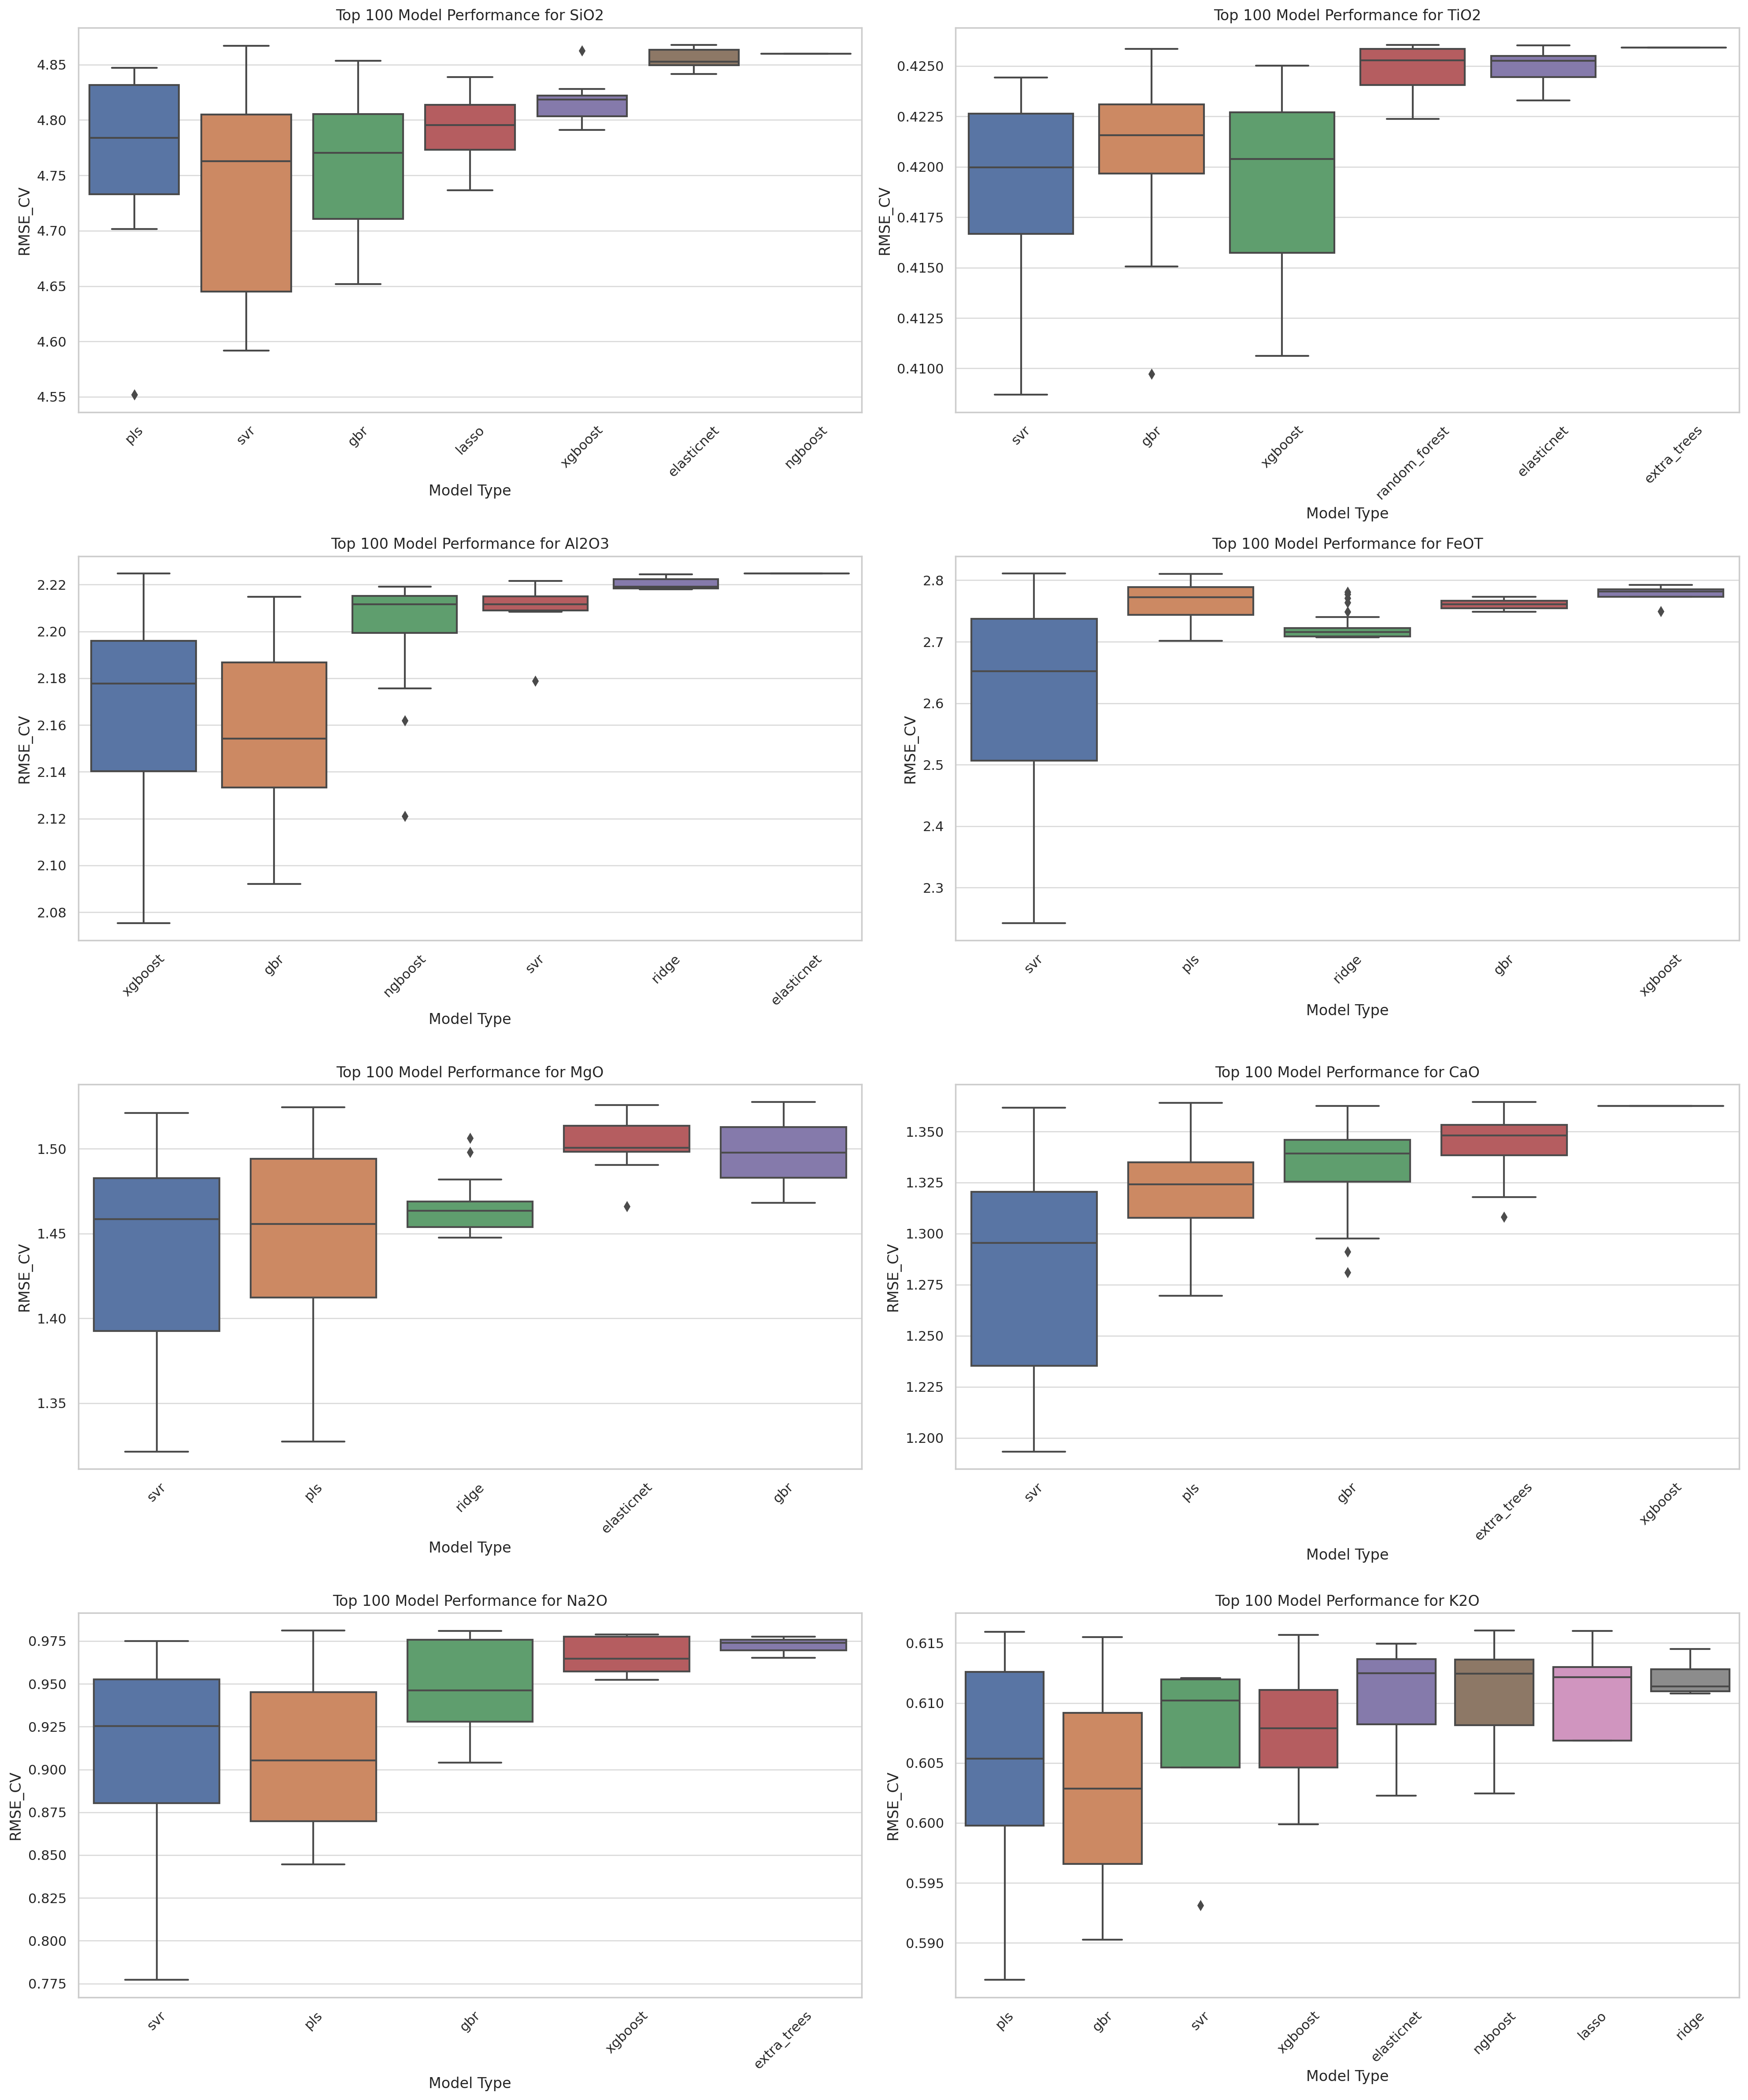
\includegraphics[width=\textwidth]{images/top100/models.png}
    \caption{Top 100 Model Performance Across Oxides. The subplots show the distribution of \gls{rmsecv} values for the top 100 trials for each model type across the eight different oxides. This helps identify the most effective models for each oxide within the top-performing trials.}
    \label{fig:top100_models}
\end{figure*}

\begin{figure*}
    \centering
    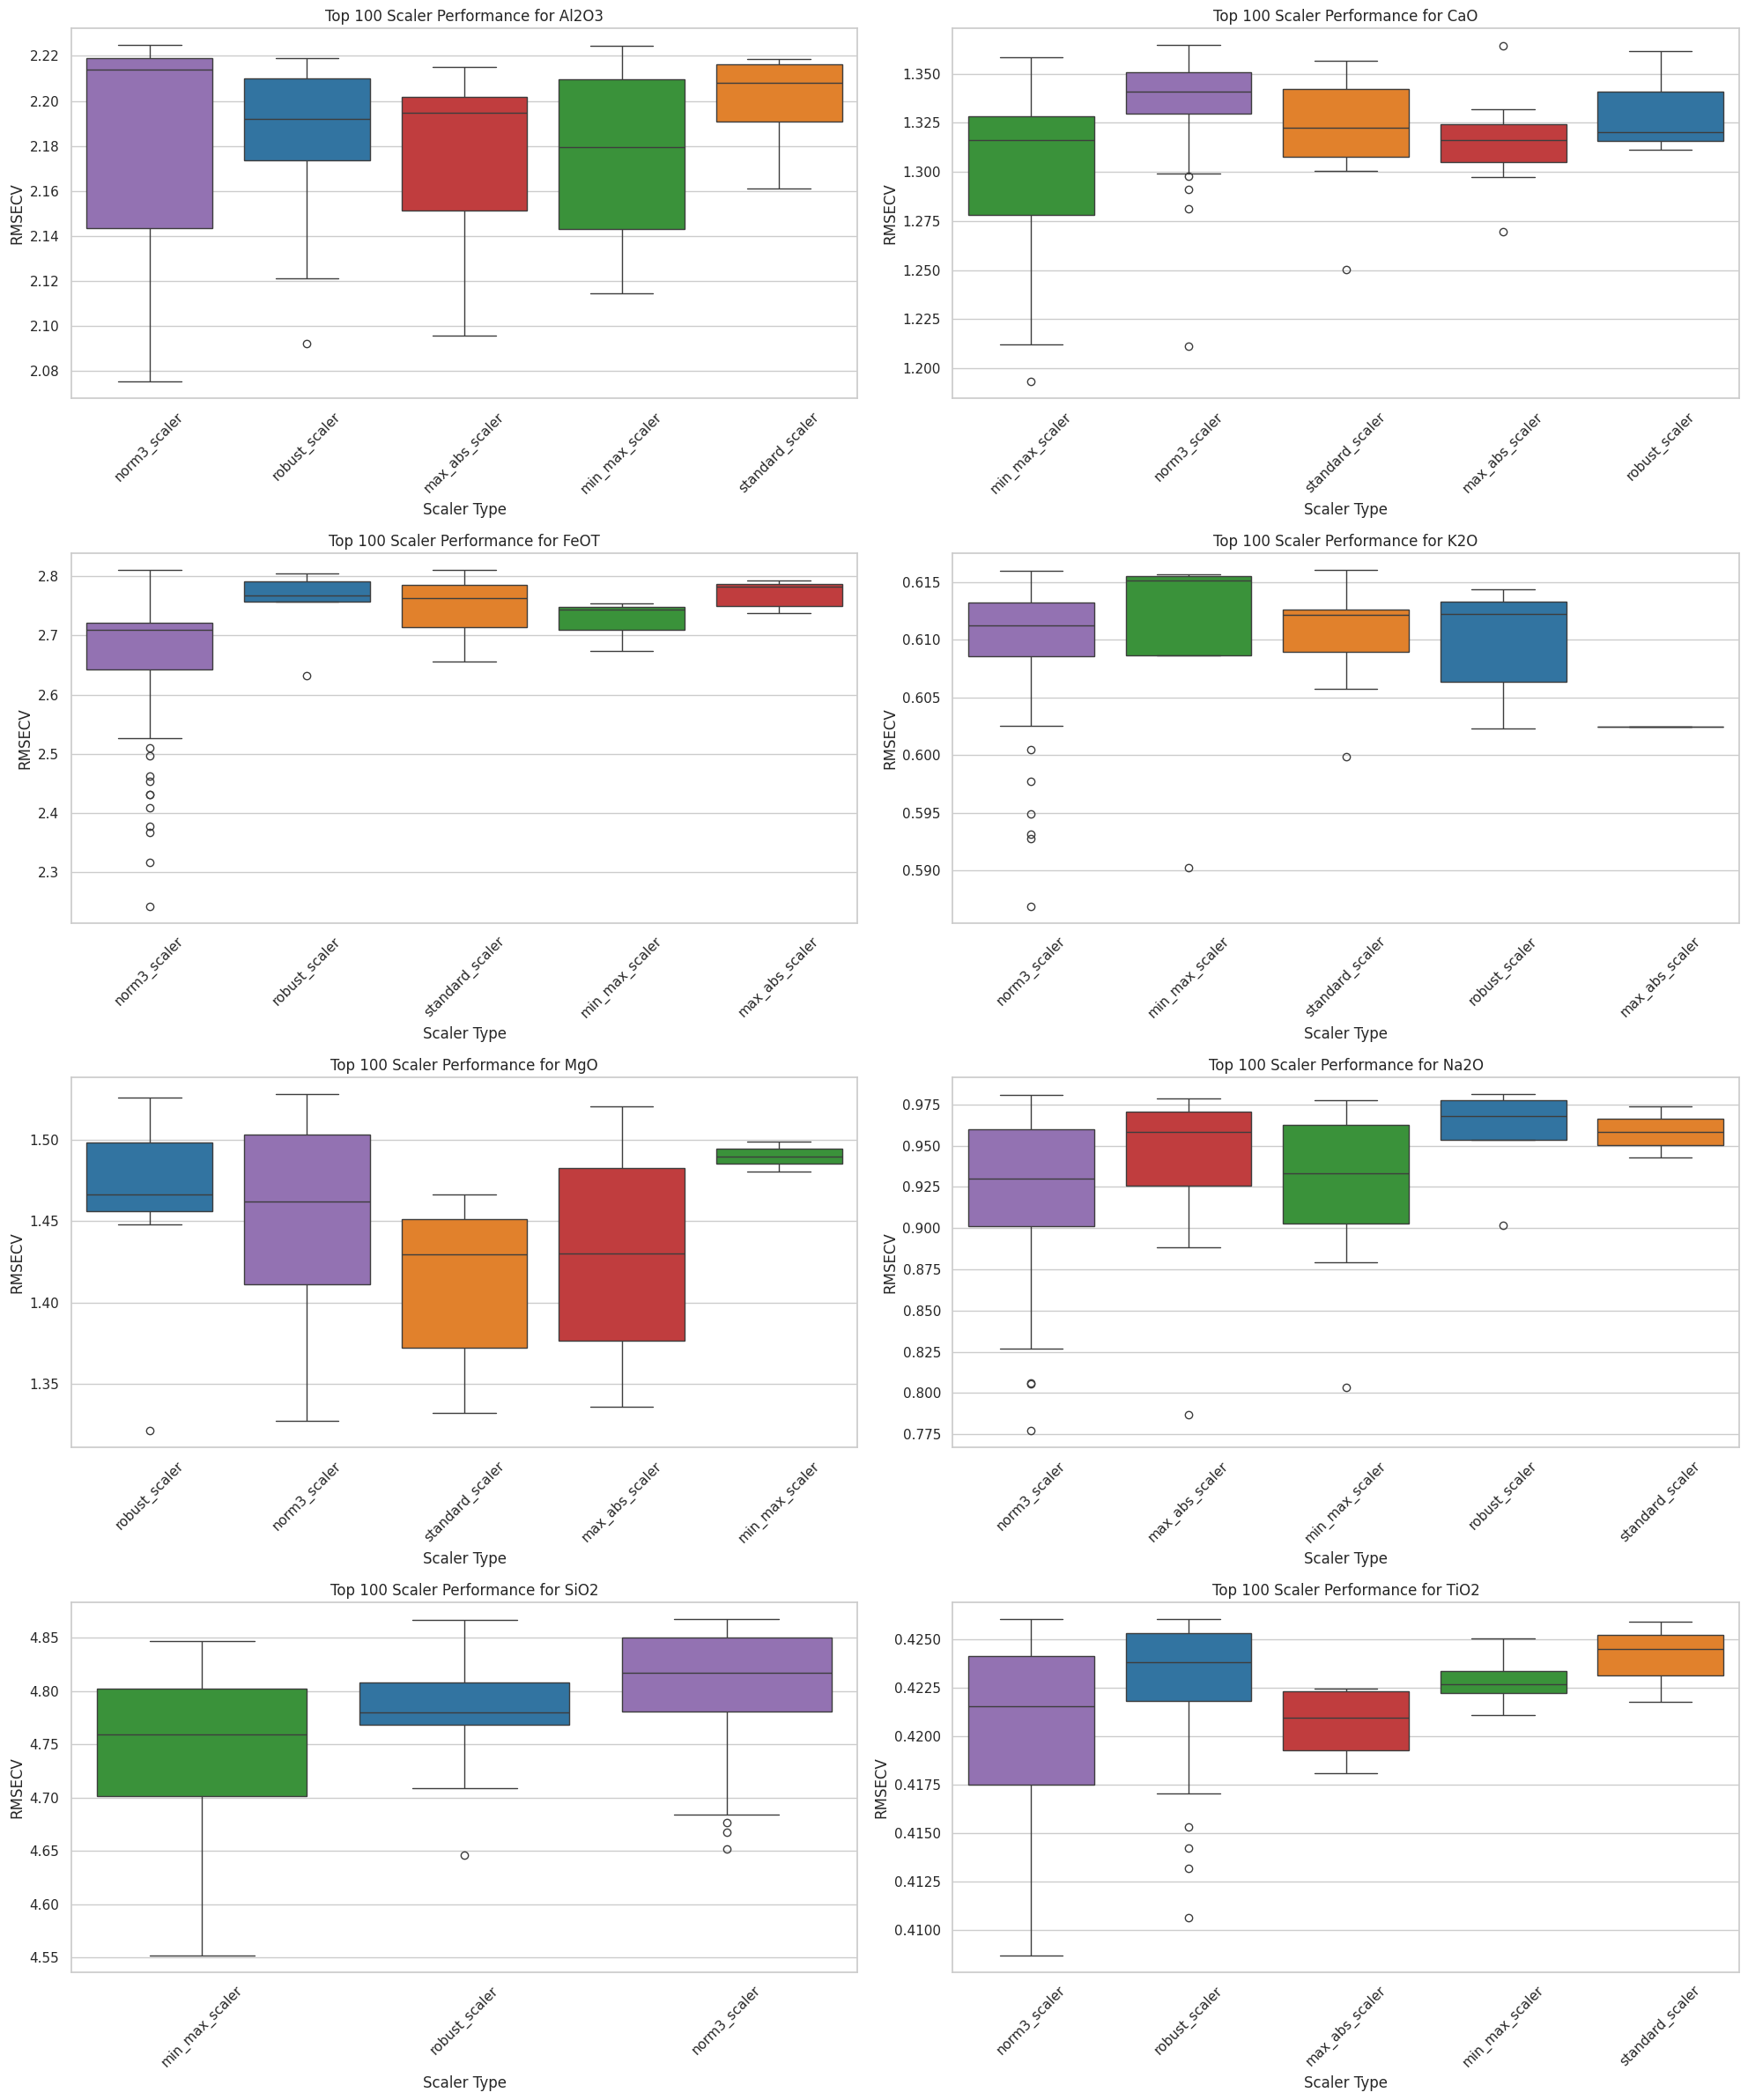
\includegraphics[width=\textwidth]{images/top100/scalers.png}
    \caption{Top 100 Scaler Performance Across Oxides. The subplots illustrate the distribution of \gls{rmsecv} values for the top 100 trials for each scaler type across the different oxides. This helps pinpoint which scalers perform best within the top-performing trials.}
    \label{fig:top100_scalers}
\end{figure*}

\begin{figure*}
    \centering
    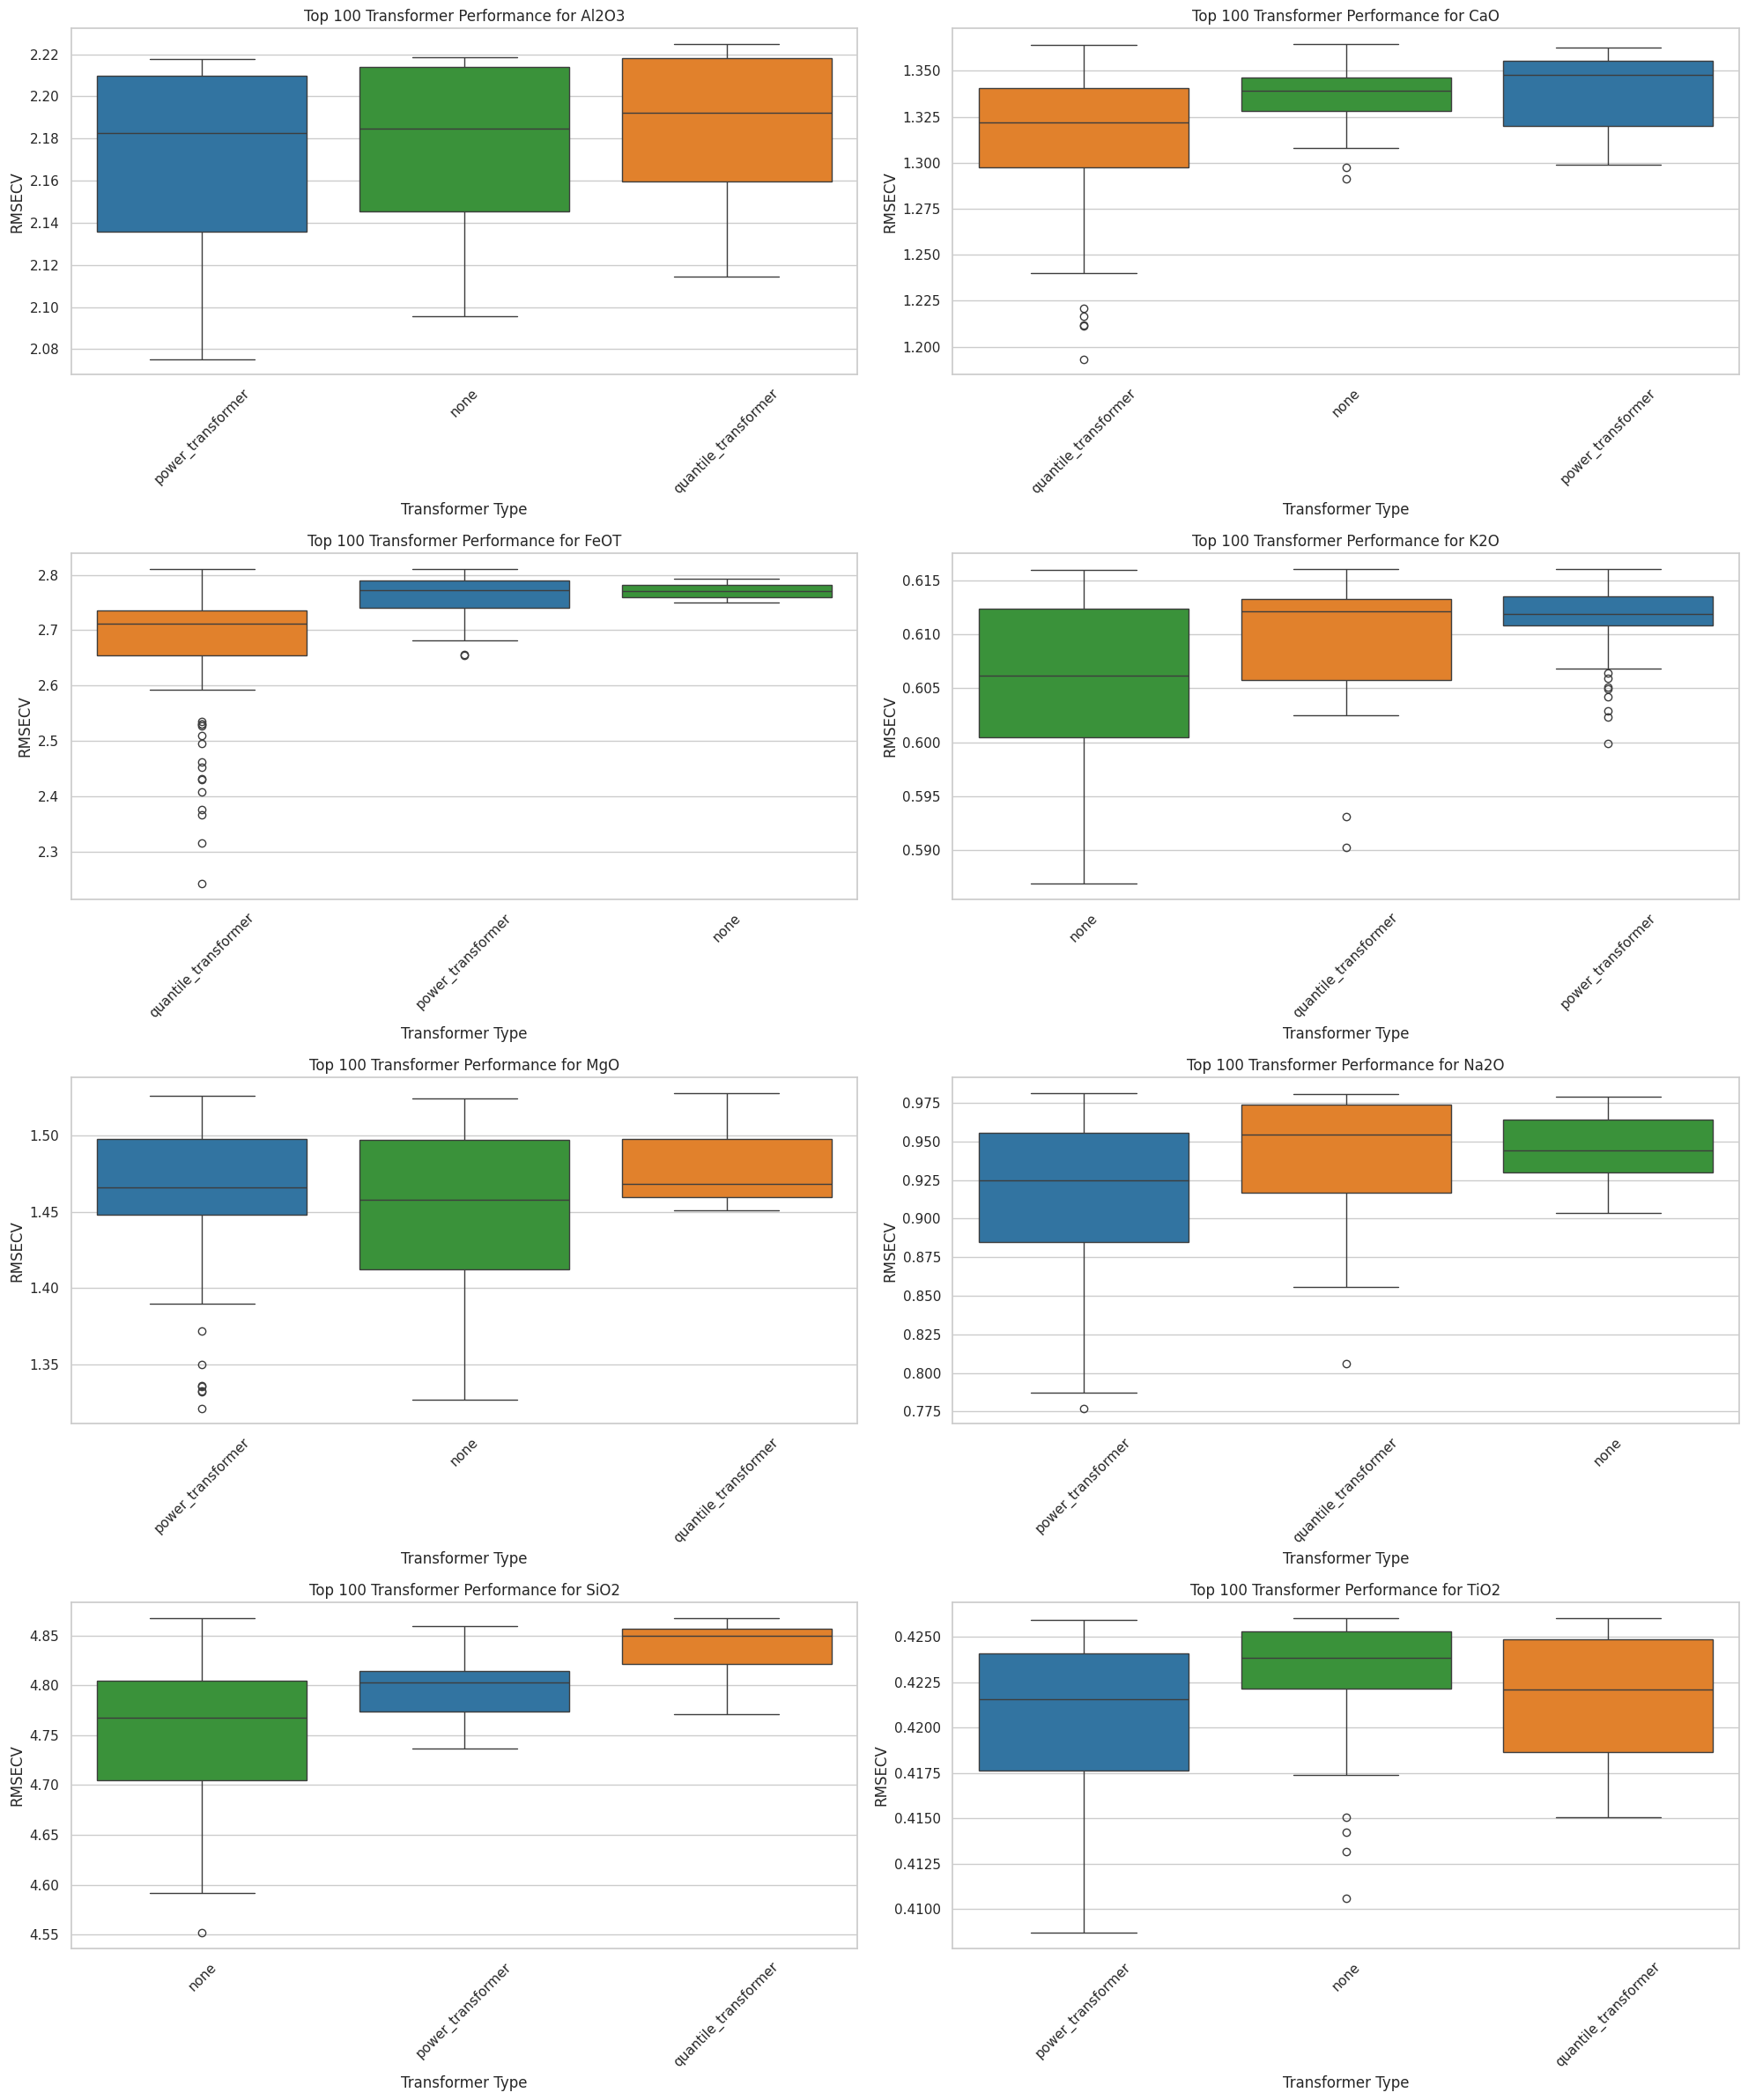
\includegraphics[width=\textwidth]{images/top100/transformers.png}
    \caption{Top 100 Transformer Performance Across Oxides. The subplots display the distribution of \gls{rmsecv} values for the top 100 trials for each transformer type across the different oxides. This helps determine the effectiveness of each transformer for different oxides within the top-performing trials.}
    \label{fig:top100_transformers}
\end{figure*}

\begin{figure*}
    \centering
    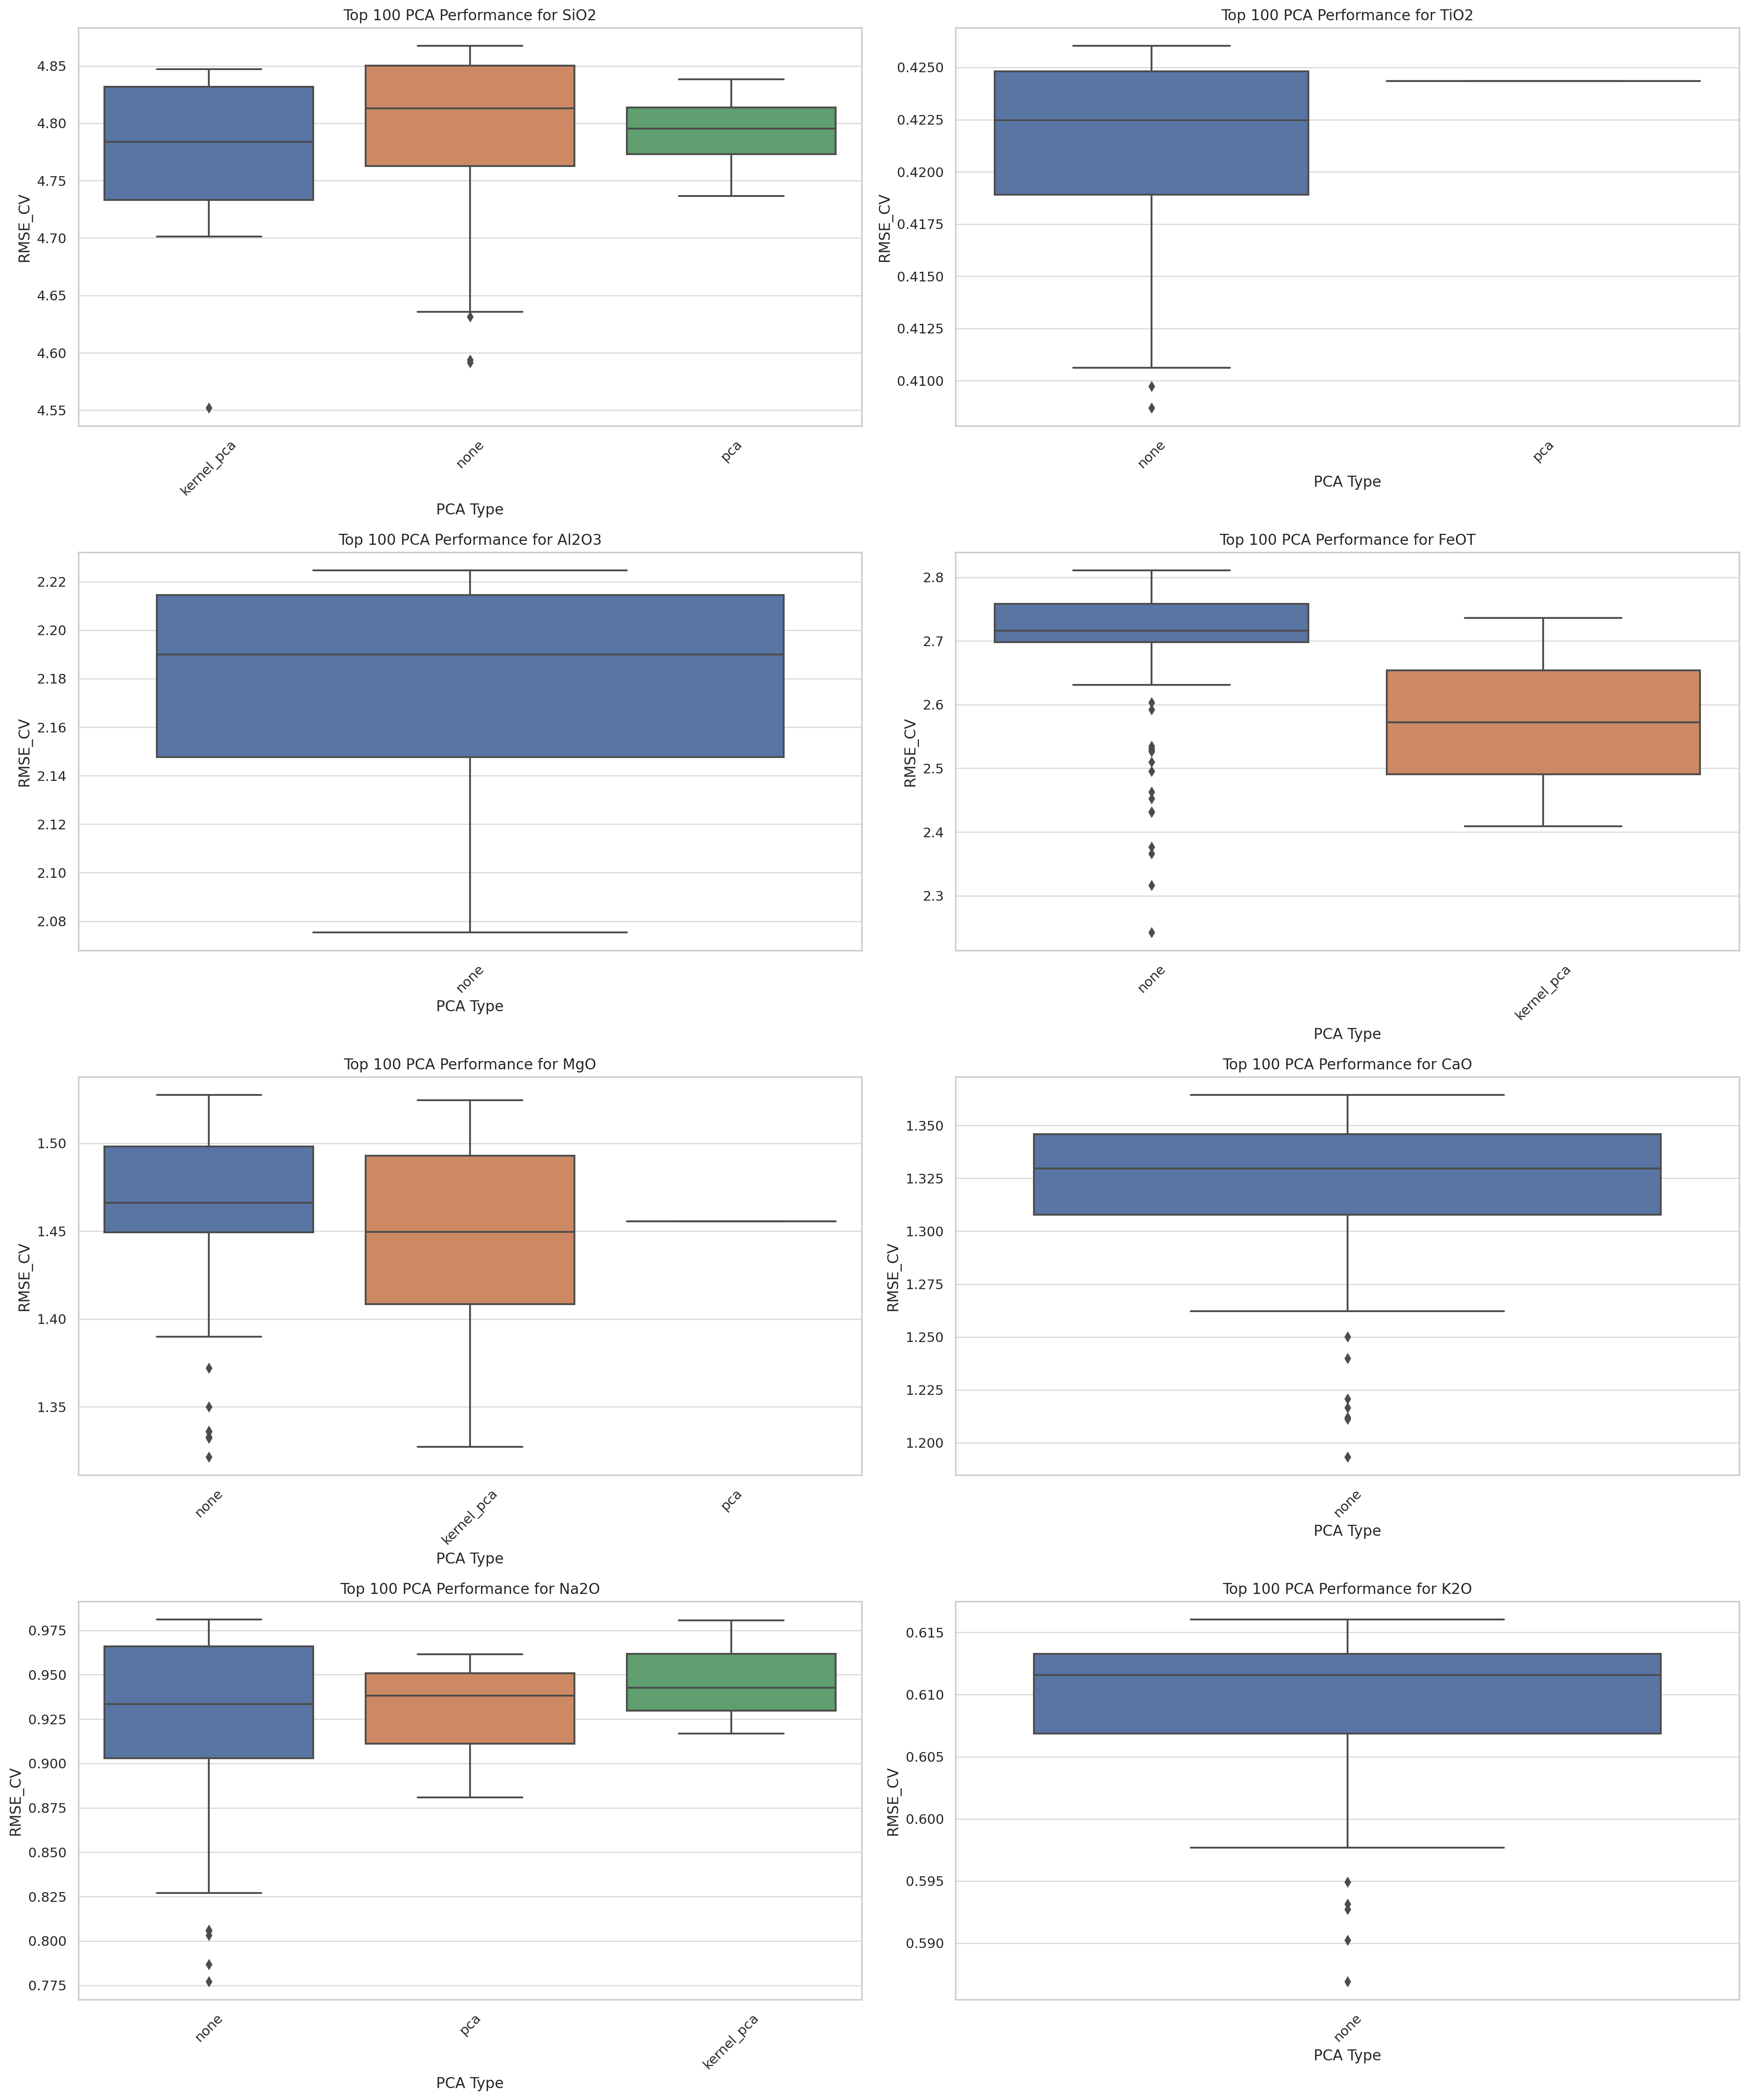
\includegraphics[width=\textwidth]{images/top100/pca.png}
    \caption{Top 100 \gls{pca} Performance Across Oxides. The subplots present the distribution of \gls{rmsecv} values for the top 100 trials for each \gls{pca} type across the different oxides. This allows us to understand the impact of \gls{pca} techniques on model performance for each oxide within the top-performing trials.}
    \label{fig:top100_pca}
\end{figure*}